\pdfminorversion=6 % this is needed to be able to include pdf 1.6. 
                    % For some reasons some old HPSG proceedings have pdf 1.6
\documentclass[11pt,a4paper,fleqn]{article}
\usepackage{times}
\thispagestyle{empty}



\usepackage[T1]{fontenc}   % Silbentrennung

\usepackage[utf8x]{inputenc}
                                                                                                                             
\hyphenation{Acad-e-my}

\usepackage[bookmarks=true,bookmarksopen=true,%
breaklinks=true,%
draft=false,plainpages=false,hyperfootnotes=false,%
pdfauthor={Stefan  Müller, Nurit Melnik (Editors)},%
pdftitle={Proceedings of the 28th International Conference on Head-Driven Phrase Structure Grammar},%
pdfkeywords={HPSG}%,
pdftex=true%
%ps2pdf=true  %ohne diesen Treiber geht der Zeilenumbruch in URLs
]{hyperref}% for pdf files
\hypersetup{colorlinks=false, pdfborder={0 0 0}}

\usepackage{pdfpages}
\pdfinclusioncopyfonts=1

\usepackage{orcidlink}

\newcommand\formatauthor[2]{\begin{tabular}[t]{@{}c@{}}
  {\LARGE#1\strut}\\
  {\small#2\strut}\\
  \rule{\dimexpr0.5\linewidth-1em}{0pt}
  \end{tabular}\xhfill\ignorespaces}
\newcommand\xhfill{\hspace{1em plus 1fill}}

\begin{document}

\begin{center}
{\Large
                {\bfseries Proceedings of the 28th International Conference on\par Head-Driven Phrase Structure Grammar\par}

                \vspace{8ex}

                     Online (Frankfurt)\\[\baselineskip]

                        Stefan  M{\"u}ller, Nurit Melnik (Editors)\\[\baselineskip]

                                2021\\[\baselineskip]

%                          CSLI Publications\\[\baselineskip]

%              http://csli-publications.stanford.edu/HPSG/2021 \\[4\baselineskip]

The papers are published under a \href{http://creativecommons.org/licenses/by/4.0/}{CC-BY license}:\\[3pt]
\href{http://creativecommons.org/licenses/by/4.0/}{http://creativecommons.org/licenses/by/4.0/}
}
\end{center}
\newpage
\tableofcontents

\newpage

\section*{Editor's note}
\addcontentsline{toc}{section}{Editor's note}
%% -*- coding:utf-8 -*-
The 27th International Conference on Head-Driven Phrase Structure Grammar (2020) was planned to take
place in Leuven (organized by Frank Van Eynde and Liesbeth Augustinus), but due to the Corona
pandemic it was organized online by Stefan Müller (Humboldt Universität zu Berlin) and Olga
Zamaraeva (University of Washington, Seattle).


The conference featured 3 invited talks and 11 papers selected by the program committee 
(Anne Abeillé, 
    Doug Arnold,
    Emily Bender,
    Felix Bildhauer,
    Hans Boas,
    Olivier Bonami,
    Francis Bond, 
    Gosse Bouma, 
    Antonio Branco, 
    Rui Chaves, 
    Philippa Cook, 
    Berthold Crysmann,
    Dan Flickinger, 
    Antske Fokkens, 
    Petter Haugereid, 
    Fabiola Henri, 
    Thomas Hoffmann, 
    Anke Holler (chair),
    Gianina Iordăchioaia,
    Paul Kay, 
    Jong-Bok Kim, 
    Jean-Pierre Koenig, 
    David Lahm, 
    Bob Levine, 
    Nurit Melnik, 
    Laura Michaelis, 
    Philip Miller, 
    Stefan Müller, 
    Tsuneko Nakazawa, 
    Petya Osenova, 
    Rainer Osswald, 
    Gerald Penn, 
    Frank Richter, 
    Louisa Sadler, 
    Manfred Sailer, 
    Pollet Samvellian, 
    Jesse Tseng, 
    Stephen Wechsler, 
    Eun-Jung Yoo, 
    Shûichi Yatabe).


% wie viele?
%In total there were x  submissions to the conference and x submissions to the workshop.
We want to thank the program committee for putting this nice program together.

% Thanks go to Gabriela Bîlbîie and Emil Ionescu, who were in charge of local
% arrangements.
 

As in the past years the contributions to the conference proceedings are based on the five page abstract
that was reviewed by the %respective 
program committee, but there is no additional reviewing of the
longer contribution to the proceedings. To ensure easy access and fast publication we have chosen an electronic format.

The proceedings include all the papers of the conference except the ones by Liesbeth Augustinus, Gosse Bouma, Frank Van
Eynde \& Jong-Bok Kim, Gert Webelhuth and Shûichi Yatabe.


\newpage
        \setcounter{page}{5}
        \phantomsection
        \addcontentsline{toc}{section}{Gabriel Aguila-Multner, Berthold Crysmann: An inside-out approach to
French causatives}
\thispagestyle{empty}

\begin{center}
  {\huge\bfseries An inside-out approach to
French causatives\par}

  \bigskip

~\\
\begingroup
\setlength{\leftskip}{0pt plus 1fill}
\setlength{\rightskip}{0pt plus 1fill}
\setlength{\parindent}{0pt}
\setlength{\parfillskip}{0pt}
  \formatauthor{Gabriel Aguila-Multner}{\begin{tabular}{@{}c@{}}Université de Paris, Laboratoire de linguistique formelle, CNRS\end{tabular}}
\formatauthor{Berthold Crysmann}{\begin{tabular}{@{}c@{}}Université de Paris, Laboratoire de linguistique formelle, CNRS\end{tabular}}

\par\endgroup

  \vspace*{8ex}

  Proceedings of the 28th International Conference on\par Head-Driven Phrase Structure Grammar

  \bigskip

  Online (Frankfurt)

  \medskip

  Stefan  Müller, Nurit Melnik (Editors)

  \medskip

  2021

  \medskip

%  CSLI Publications

  \medskip

  pages 5--25

  \medskip

%  \url{http://csli-publications.stanford.edu/HPSG/2021}
\end{center}
\vfill

\noindent
Keywords: Clitic climbing,
French, HPSG, causative, faire, periphrasis, VP structure


\vfill
\noindent
% APA Style
Aguila-Multner, Gabriel, \& Crysmann, Berthold. 2021. An inside-out approach to
French causatives. In Müller, Stefan, \& Melnik, Nurit (Eds.), \emph{{Proceedings of the 28th International Conference on Head-Driven Phrase Structure Grammar, Online (Frankfurt)}},
5--25. DOI: \href{http://doi.org/10.21248/hpsg.2021.1}{10.21248/hpsg.2021.1}. \hfill\href{http://creativecommons.org/licenses/by/4.0/}{
\includegraphics[height=.75em]{Includes/ccby-eps-converted-to.pdf}}

\newpage
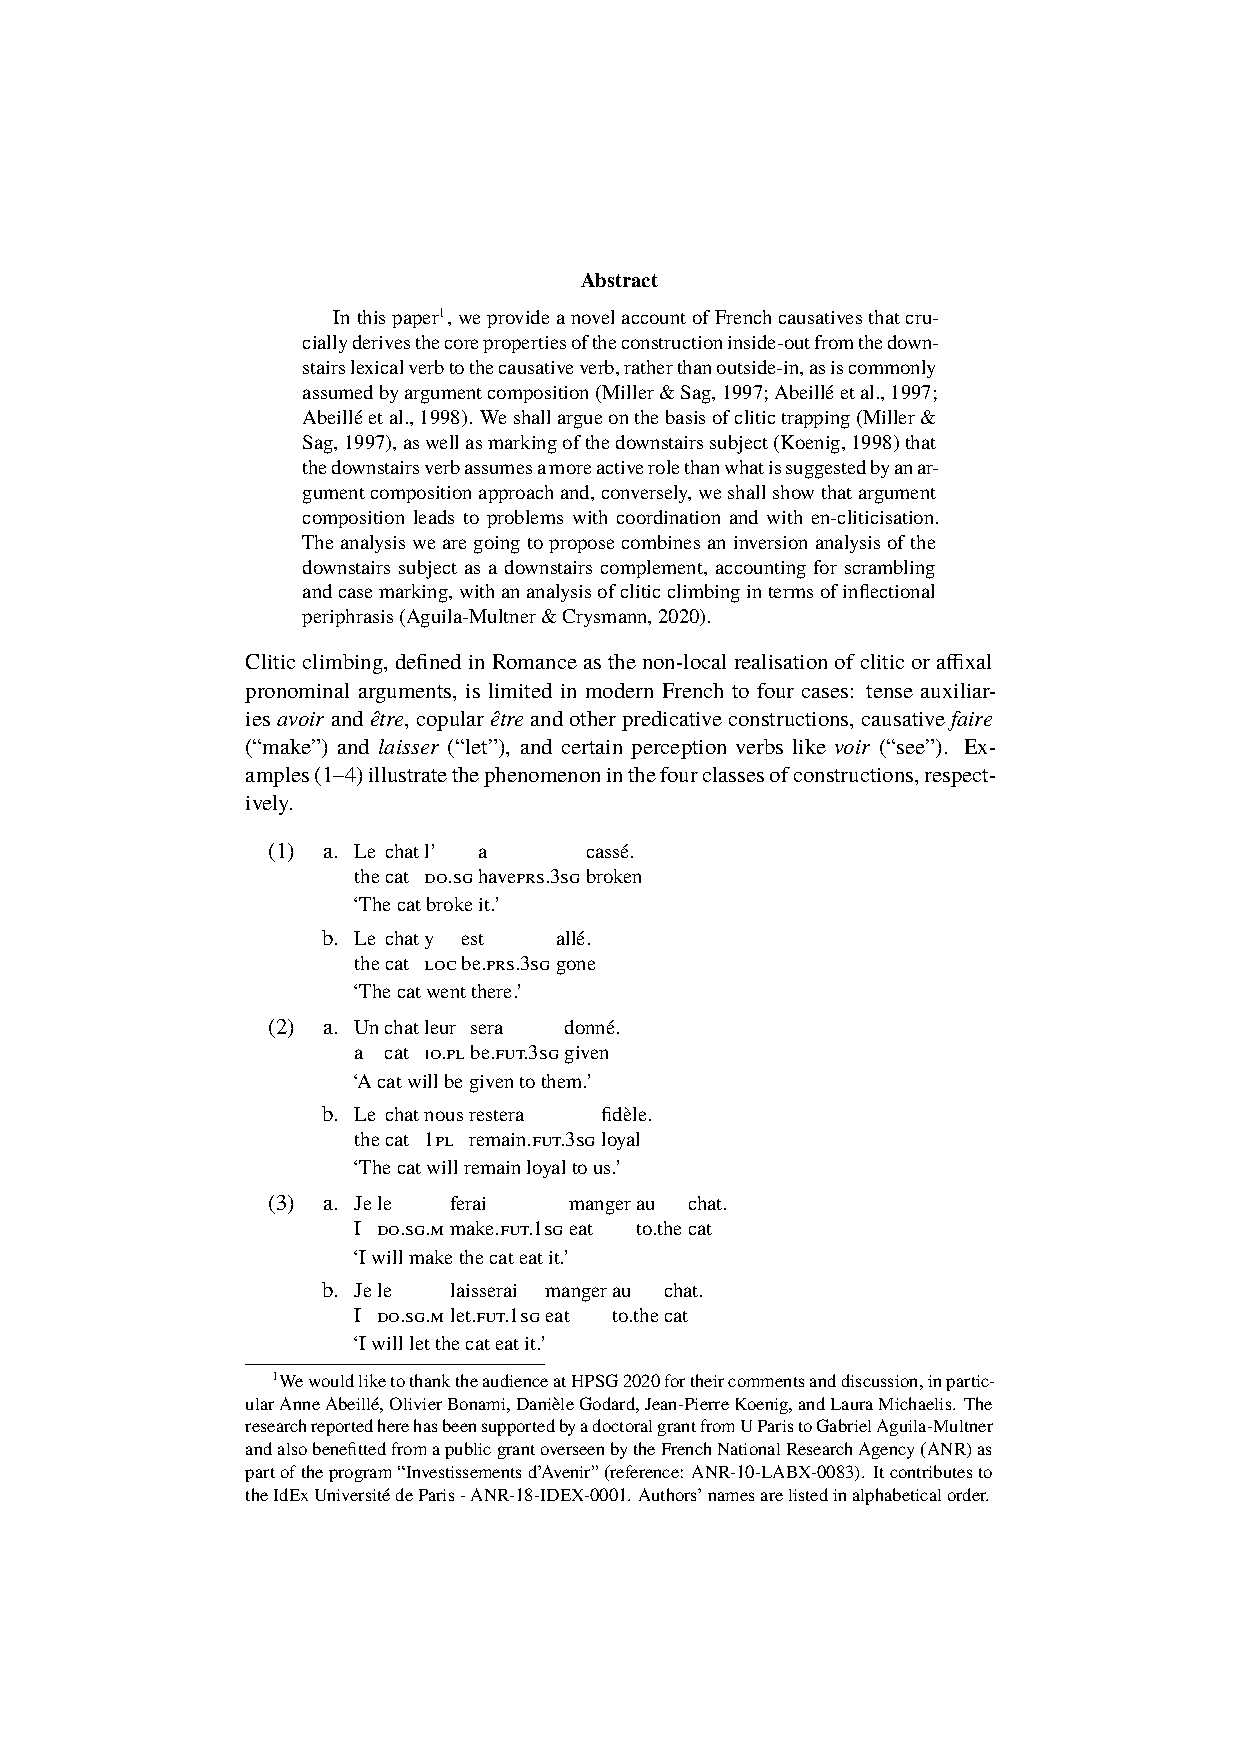
\includepdf[pages=-,pagecommand=\thispagestyle{plain}]{Includes/aguila-multner-crysmann.pdf}
        \setcounter{page}{26}
        \phantomsection
        \addcontentsline{toc}{section}{Manfred Sailer, Annika D{\"o}rner: A
Smurf-based Approach to Placeholder Expressions}
\thispagestyle{empty}

\begin{center}
  {\huge\bfseries A
Smurf-based Approach to Placeholder Expressions\par}

  \bigskip

~\\
\begingroup
\setlength{\leftskip}{0pt plus 1fill}
\setlength{\rightskip}{0pt plus 1fill}
\setlength{\parindent}{0pt}
\setlength{\parfillskip}{0pt}
  \formatauthor{Manfred Sailer}{\begin{tabular}{@{}c@{}}Goethe-University Frankfurt a.M.\end{tabular}}
\formatauthor{Annika Dörner}{\begin{tabular}{@{}c@{}}University of Erfurt\end{tabular}}

\par\endgroup

  \vspace*{8ex}

  Proceedings of the 28th International Conference on\par Head-Driven Phrase Structure Grammar

  \bigskip

  Online (Frankfurt)

  \medskip

  Stefan  Müller, Nurit Melnik (Editors)

  \medskip

  2021

  \medskip

%  CSLI Publications

  \medskip

  pages 26--46

  \medskip

%  \url{http://csli-publications.stanford.edu/HPSG/2021}
\end{center}
\vfill

\noindent
Keywords: German, HPSG, morphology, placeholder expression, smurfing


\vfill
\noindent
% APA Style
Sailer, Manfred, \& Dörner, Annika. 2021. A
Smurf-based Approach to Placeholder Expressions. In Müller, Stefan, \& Melnik, Nurit (Eds.), \emph{{Proceedings of the 28th International Conference on Head-Driven Phrase Structure Grammar, Online (Frankfurt)}},
26--46. DOI: \href{http://doi.org/10.21248/hpsg.2021.2}{10.21248/hpsg.2021.2}. \hfill\href{http://creativecommons.org/licenses/by/4.0/}{
\includegraphics[height=.75em]{Includes/ccby-eps-converted-to.pdf}}

\newpage
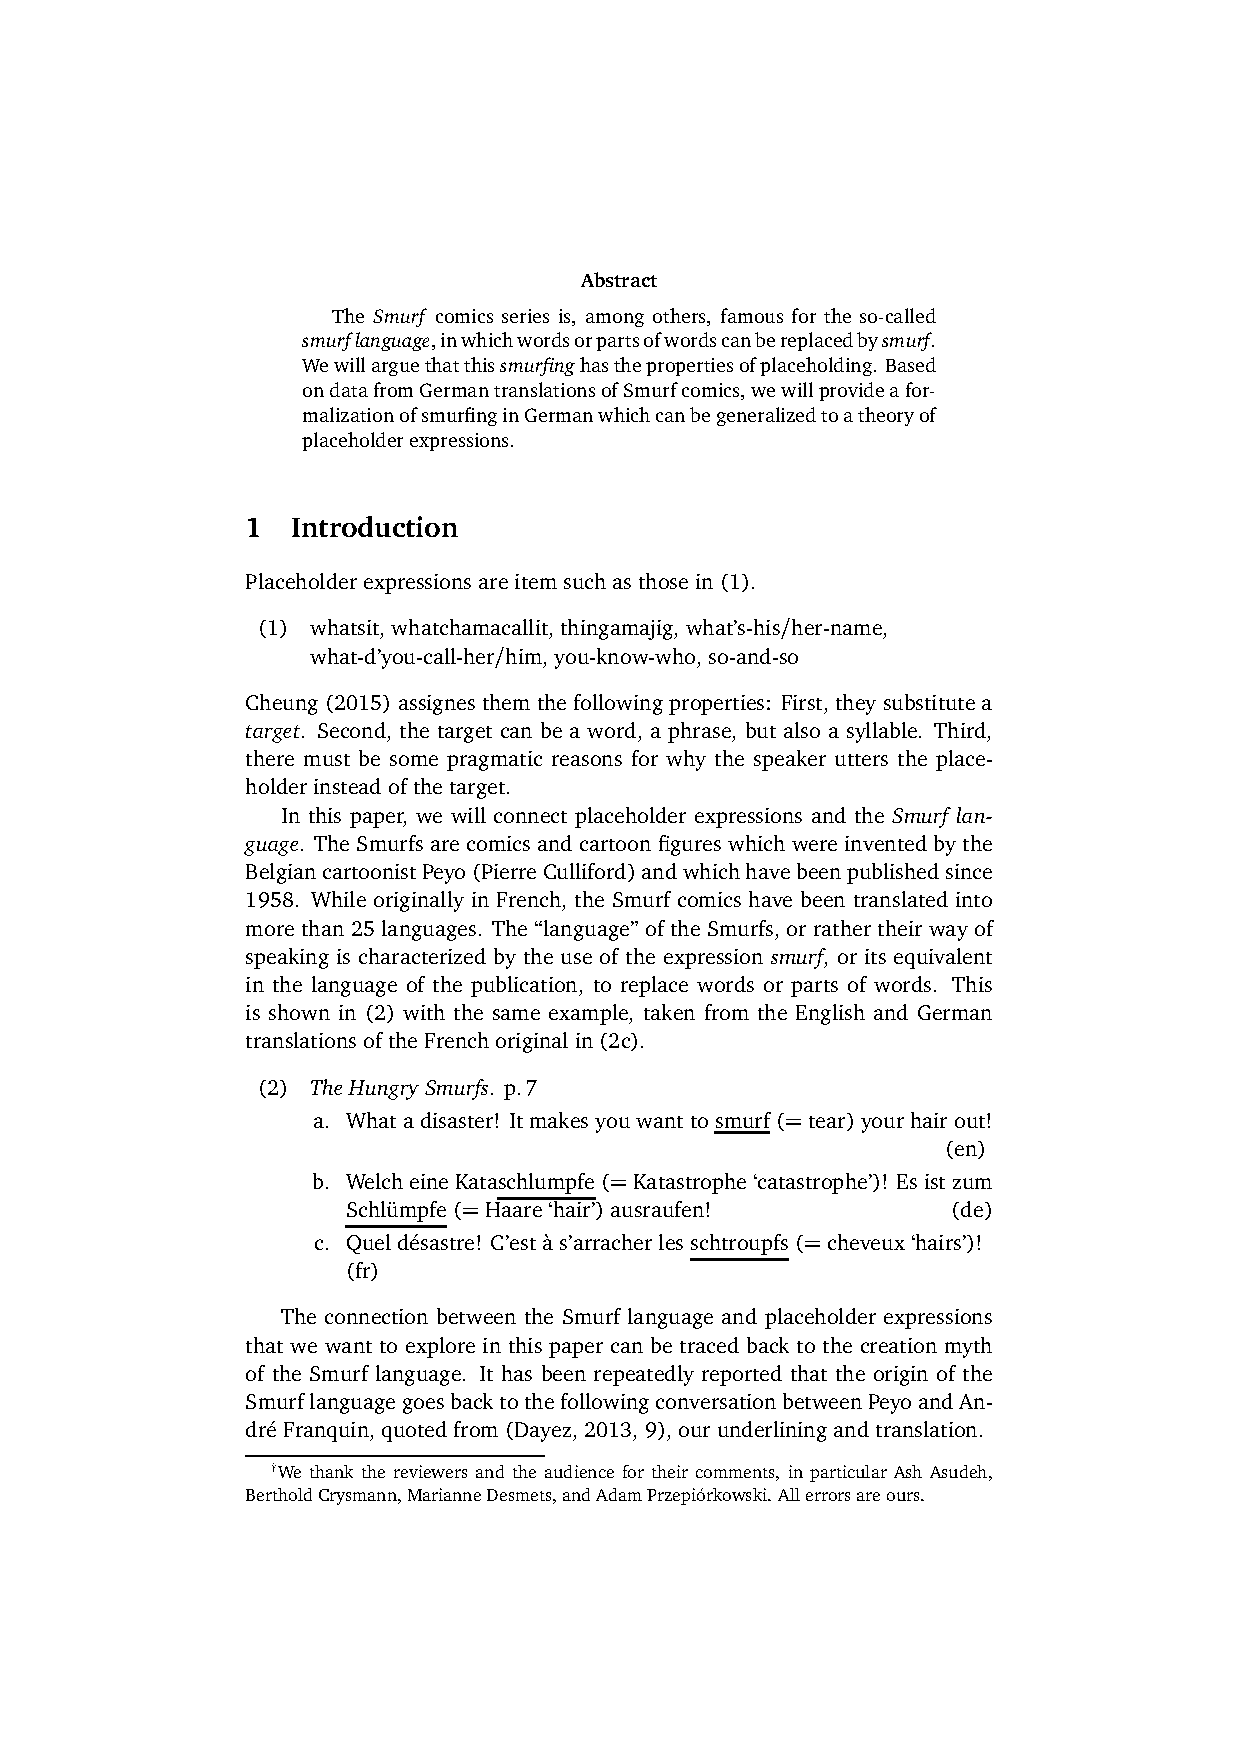
\includepdf[pages=-,pagecommand=\thispagestyle{plain}]{Includes/sailer-doerner.pdf}
        \setcounter{page}{47}
        \phantomsection
        \addcontentsline{toc}{section}{Yanru Lu, Stefan M{\"u}ller: Verbal reduplication in Mandarin Chinese: An HPSG account}
\thispagestyle{empty}

\begin{center}
  {\huge\bfseries Verbal reduplication in Mandarin Chinese: An HPSG account\par}

  \bigskip

~\\
\begingroup
\setlength{\leftskip}{0pt plus 1fill}
\setlength{\rightskip}{0pt plus 1fill}
\setlength{\parindent}{0pt}
\setlength{\parfillskip}{0pt}
  \formatauthor{Yanru Lu}{\begin{tabular}{@{}c@{}}Humboldt-Universität zu Berlin\end{tabular}}
\formatauthor{Stefan Müller\,\orcidlink{0000-0003-4413-5313}}{\begin{tabular}{@{}c@{}}Humboldt-Universität zu Berlin\end{tabular}}

\par\endgroup

  \vspace*{8ex}

  Proceedings of the 28th International Conference on\par Head-Driven Phrase Structure Grammar

  \bigskip

  Online (Frankfurt)

  \medskip

  Stefan  Müller, Nurit Melnik (Editors)

  \medskip

  2021

  \medskip

%  CSLI Publications

  \medskip

  pages 47--67

  \medskip

%  \url{http://csli-publications.stanford.edu/HPSG/2021}
\end{center}
\vfill

\noindent
Keywords: Chinese, HPSG, reduplication


\vfill
\noindent
% APA Style
Lu, Yanru, \& Müller, Stefan. 2021. Verbal reduplication in Mandarin Chinese: An HPSG account. In Müller, Stefan, \& Melnik, Nurit (Eds.), \emph{{Proceedings of the 28th International Conference on Head-Driven Phrase Structure Grammar, Online (Frankfurt)}},
47--67. DOI: \href{http://doi.org/10.21248/hpsg.2021.3}{10.21248/hpsg.2021.3}. \hfill\href{http://creativecommons.org/licenses/by/4.0/}{
\includegraphics[height=.75em]{Includes/ccby-eps-converted-to.pdf}}

\newpage
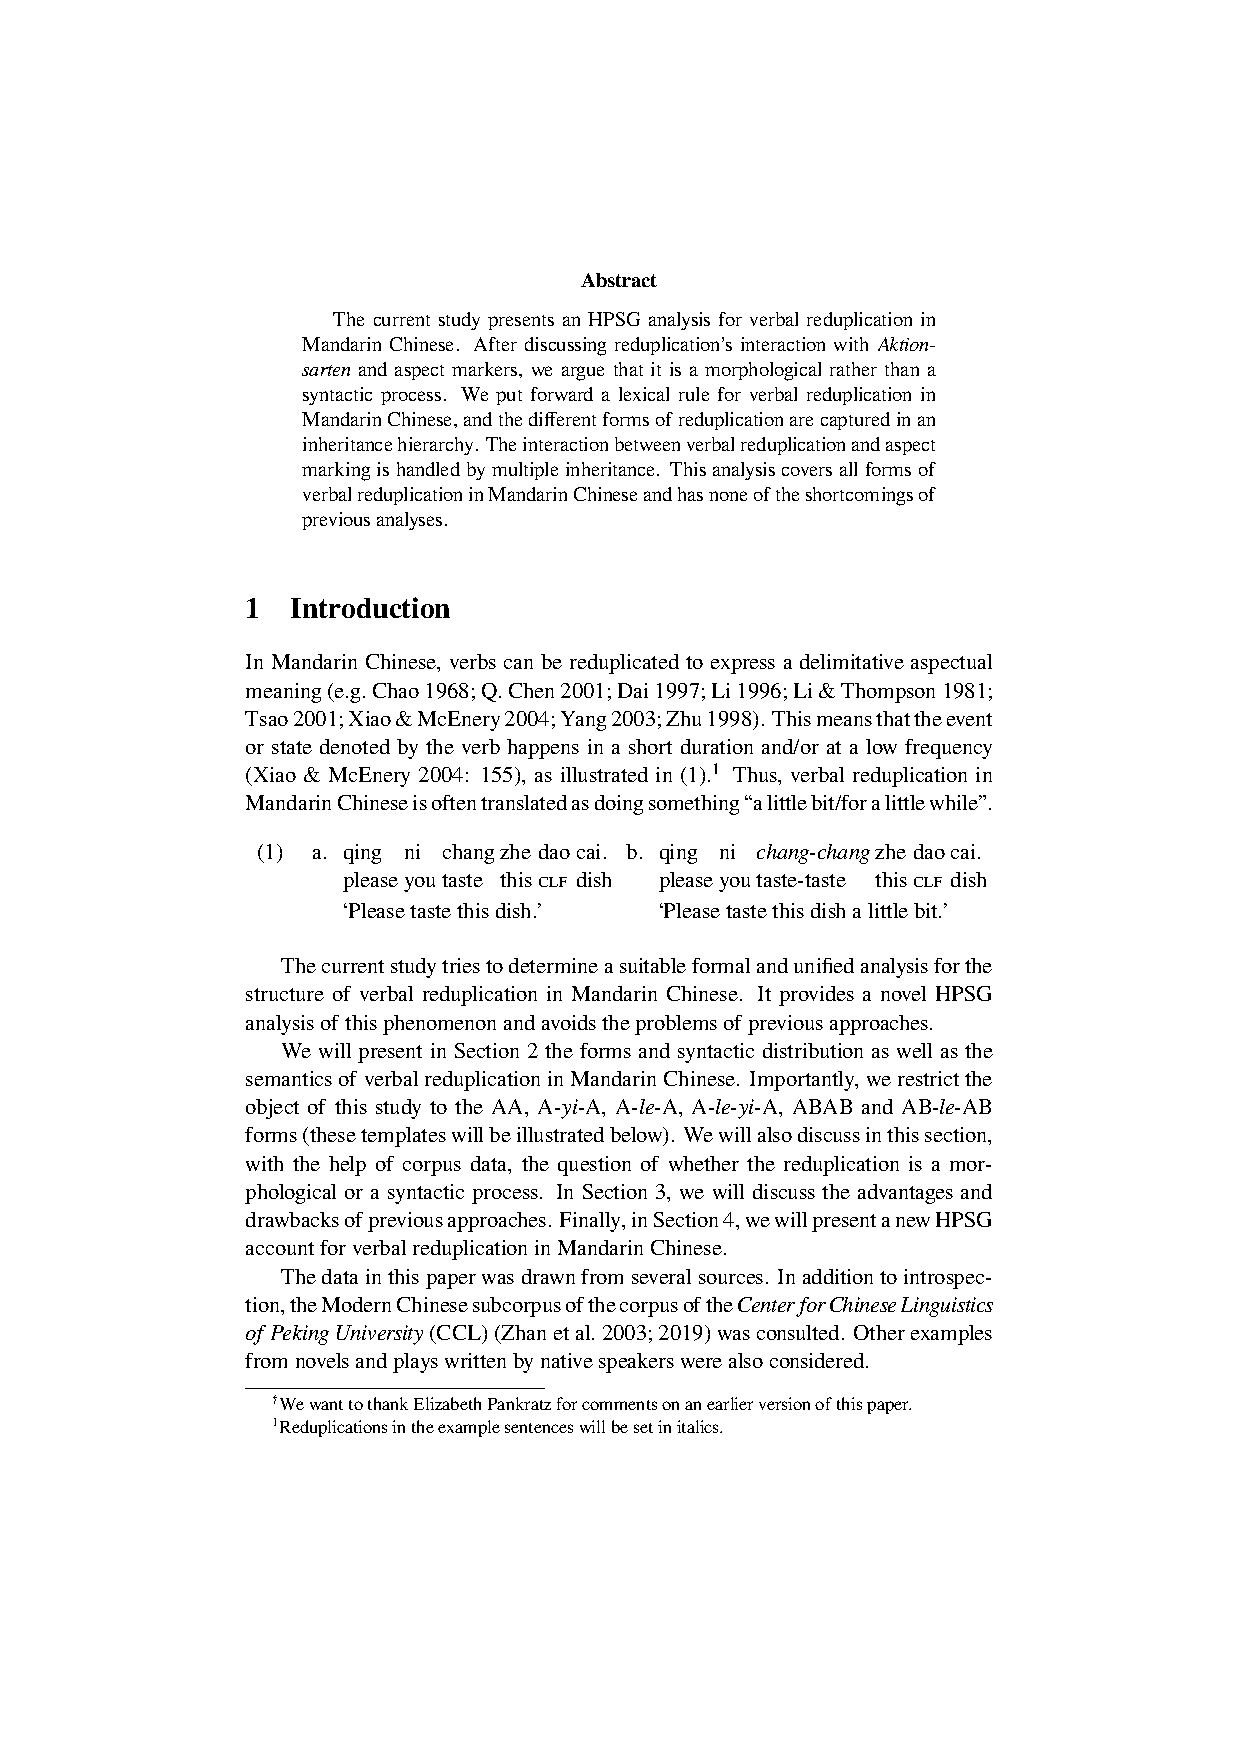
\includepdf[pages=-,pagecommand=\thispagestyle{plain}]{Includes/lu-mueller.pdf}
\end{document}
